\chapter{User Interface Design}
\section{Mockups}
The User App is the interface which permit customers to enjoy CLup services. Whether installed on a smartphone or on a ticketing kiosk, it is the only way for a customer to use CLup.
User interface mockups of most important pages of the app are shown below.

\vspace{0.5cm}
\begin{minipage}{.5\textwidth}
	\centering
	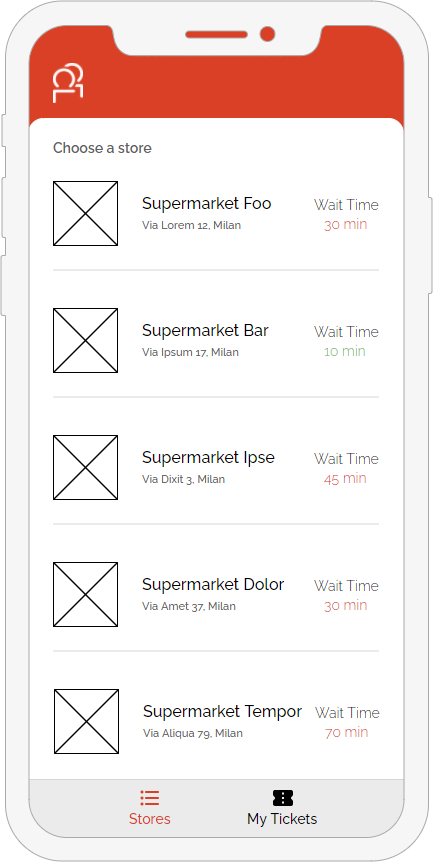
\includegraphics[scale=0.8]{home}
	\captionsetup{type=figure}
	\caption{App home.}
\end{minipage}%
\begin{minipage}{.5\textwidth}
	\centering
	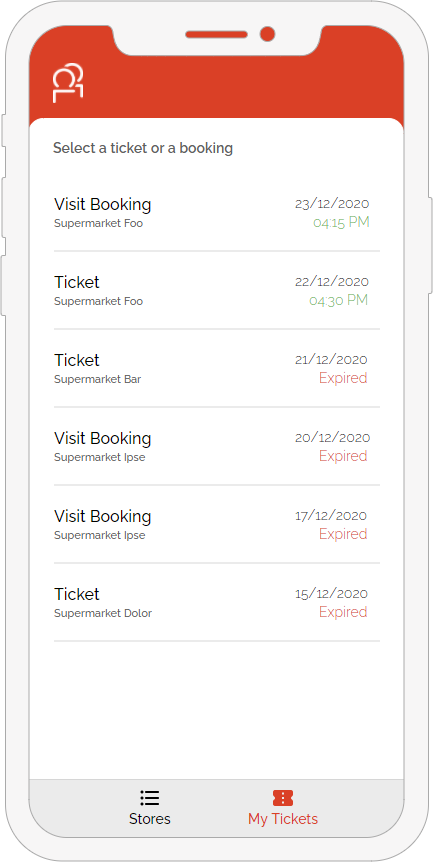
\includegraphics[scale=0.8]{my_tickets}
	\captionsetup{type=figure}
	\caption{Tickets list.}
\end{minipage}

\clearpage

\begin{minipage}{.5\textwidth}
	\centering
	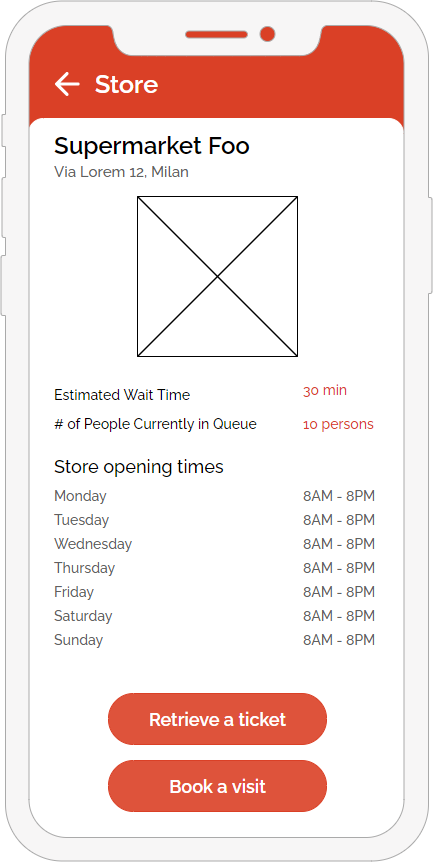
\includegraphics[scale=0.8]{store}
	\captionsetup{type=figure}
	\caption{Store page.}
\end{minipage}%
\begin{minipage}{.5\textwidth}
	\centering
	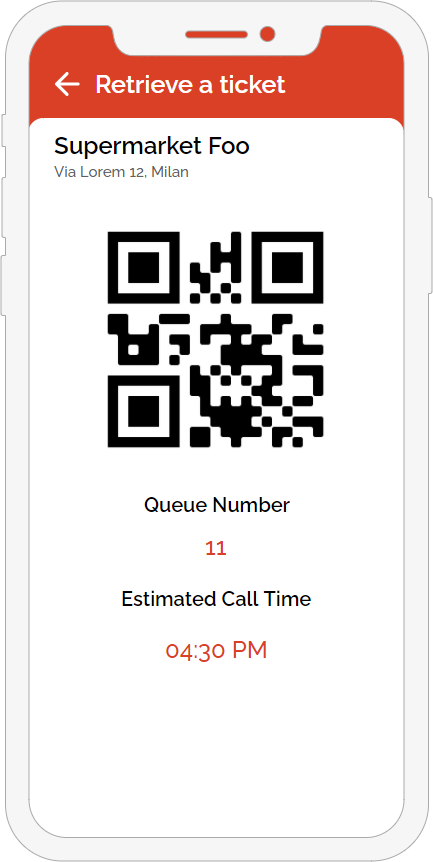
\includegraphics[scale=0.8]{ticket}
	\captionsetup{type=figure}
	\caption{Ticket Retrieved.}
\end{minipage}

\vspace{1cm}

\begin{minipage}{.5\textwidth}
	\centering
	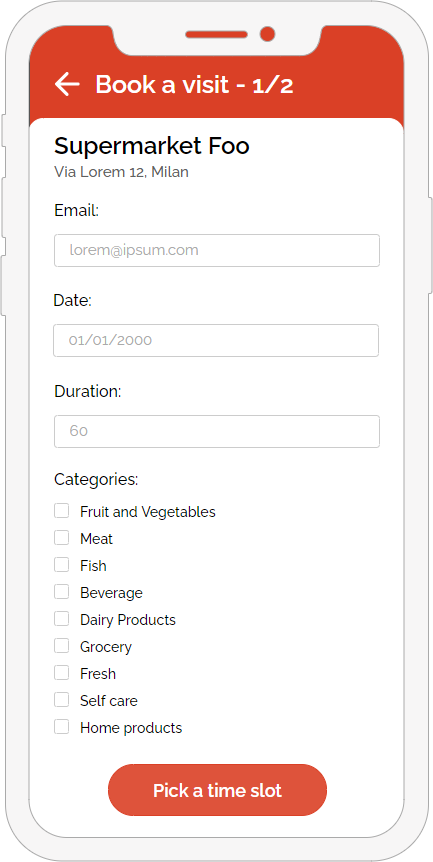
\includegraphics[scale=0.8]{book1}
	\captionsetup{type=figure}
	\caption{Book a visit (1/2).}
\end{minipage}%
\begin{minipage}{.5\textwidth}
	\centering
	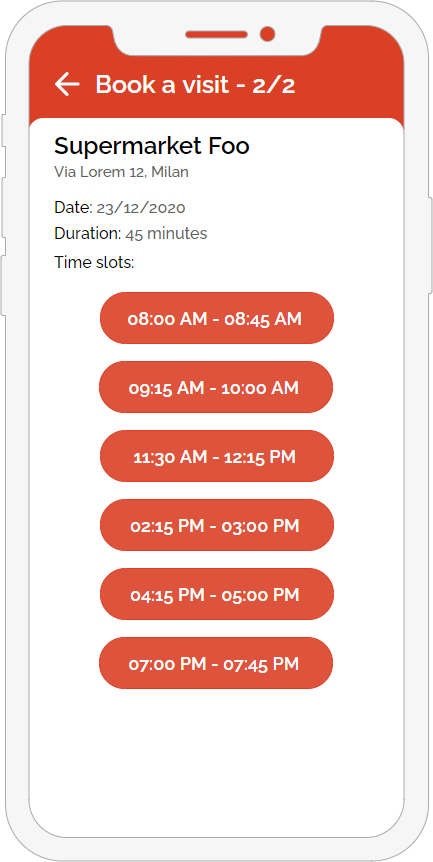
\includegraphics[scale=0.8]{book2}
	\captionsetup{type=figure}
	\caption{Book a visit (2/2).}
\end{minipage}

\vspace{1cm}

\begin{figure}[H]
	\centering
	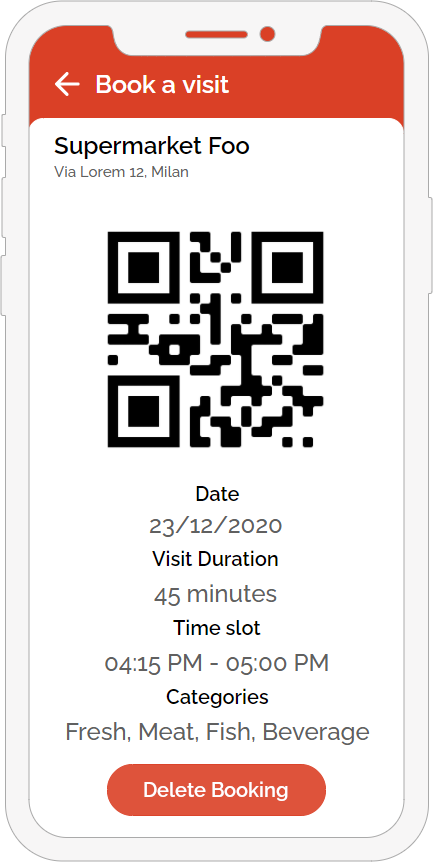
\includegraphics[scale=0.8]{book3}
	\caption{Visit booked.}
\end{figure}

\clearpage
The Store App is the interface used by employees to scan store pass QRs.
User interface mockups of most important pages of the app are shown below.
\vspace{0.5cm}

\begin{minipage}{.5\textwidth}
	\centering
	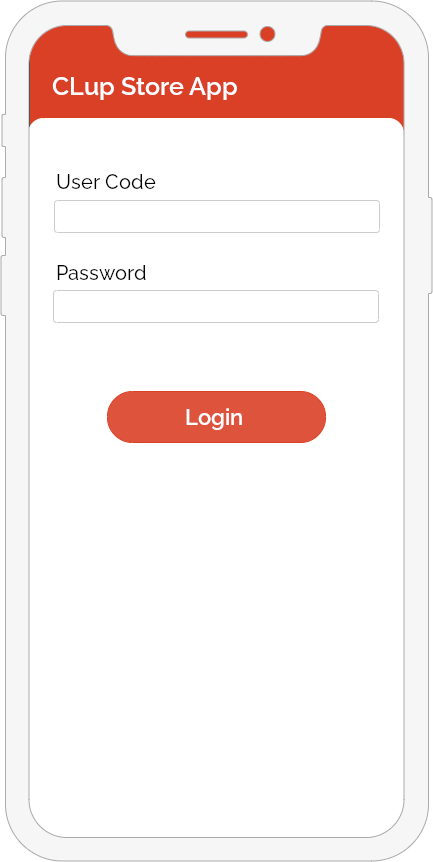
\includegraphics[scale=0.8]{login_app}
	\captionsetup{type=figure}
	\caption{Login page.}
\end{minipage}%
\begin{minipage}{.5\textwidth}
	\centering
	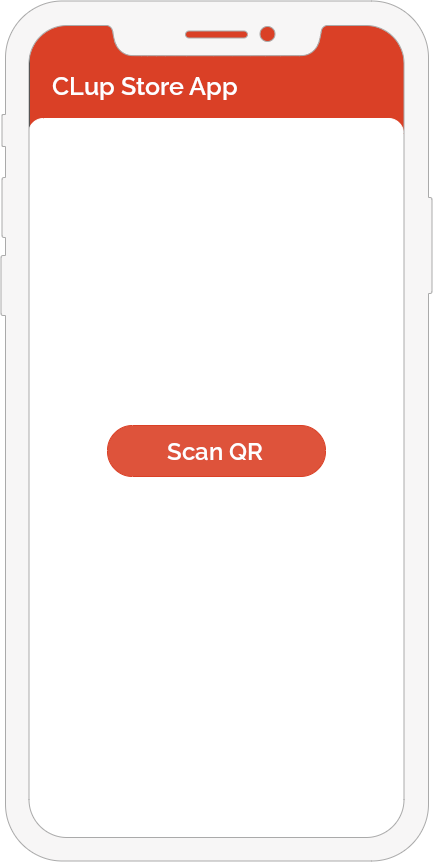
\includegraphics[scale=0.8]{scan_ticket}
	\captionsetup{type=figure}
	\caption{Home page.}
\end{minipage}

\vspace{1cm}

\begin{minipage}{.5\textwidth}
	\centering
	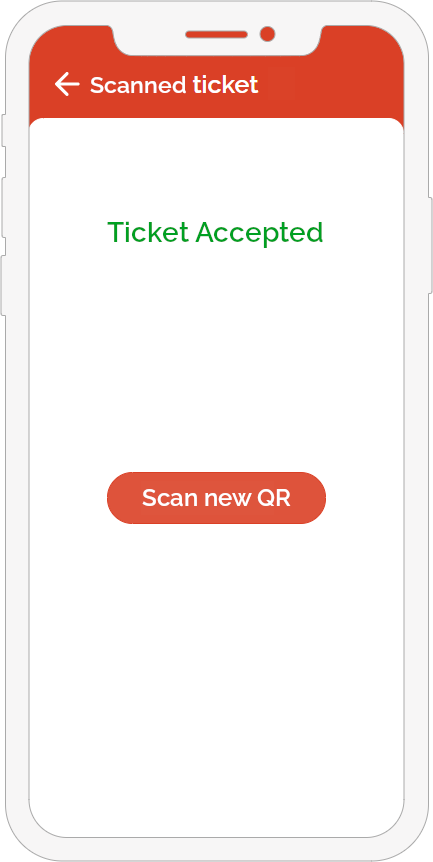
\includegraphics[scale=0.8]{ticket_scanned1}
	\captionsetup{type=figure}
	\caption{Ticket Scanned (accepted).}
\end{minipage}%
\begin{minipage}{.5\textwidth}
	\centering
	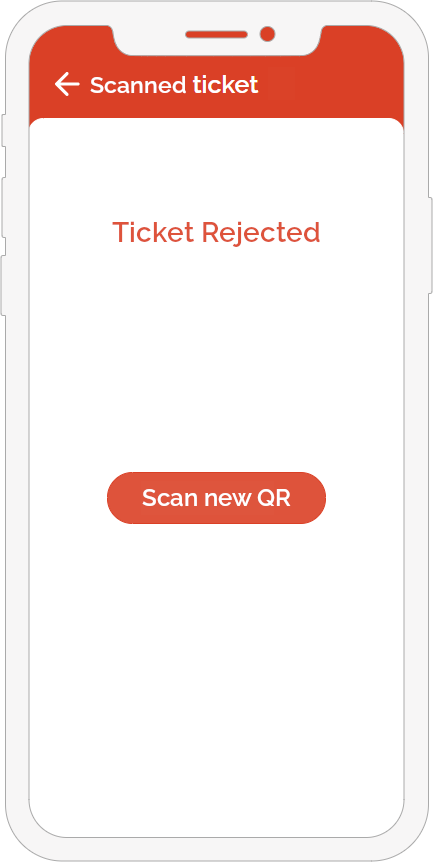
\includegraphics[scale=0.8]{ticket_scanned2}
	\captionsetup{type=figure}
	\caption{Ticket Scanned (rejected).}
\end{minipage}

\clearpage

Store managers and store employees use a web based interface for enjoying CLup features. The CLup admins can login at the same interface as well.
User interface mockups of most important pages of the web dashboard are shown below.
\vspace{0.5cm}
\begin{figure}[H]
	\centering
	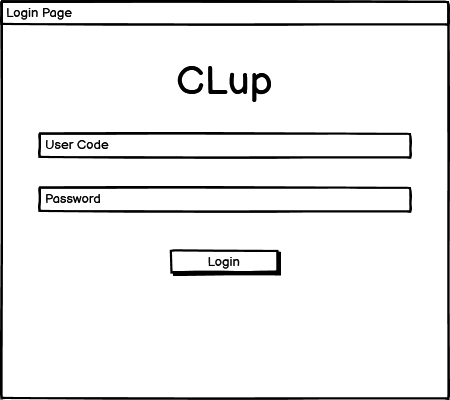
\includegraphics[width=0.64\linewidth]{login}
	\caption{Dashboard login.}
\end{figure}
\begin{figure}[H]
	\centering
	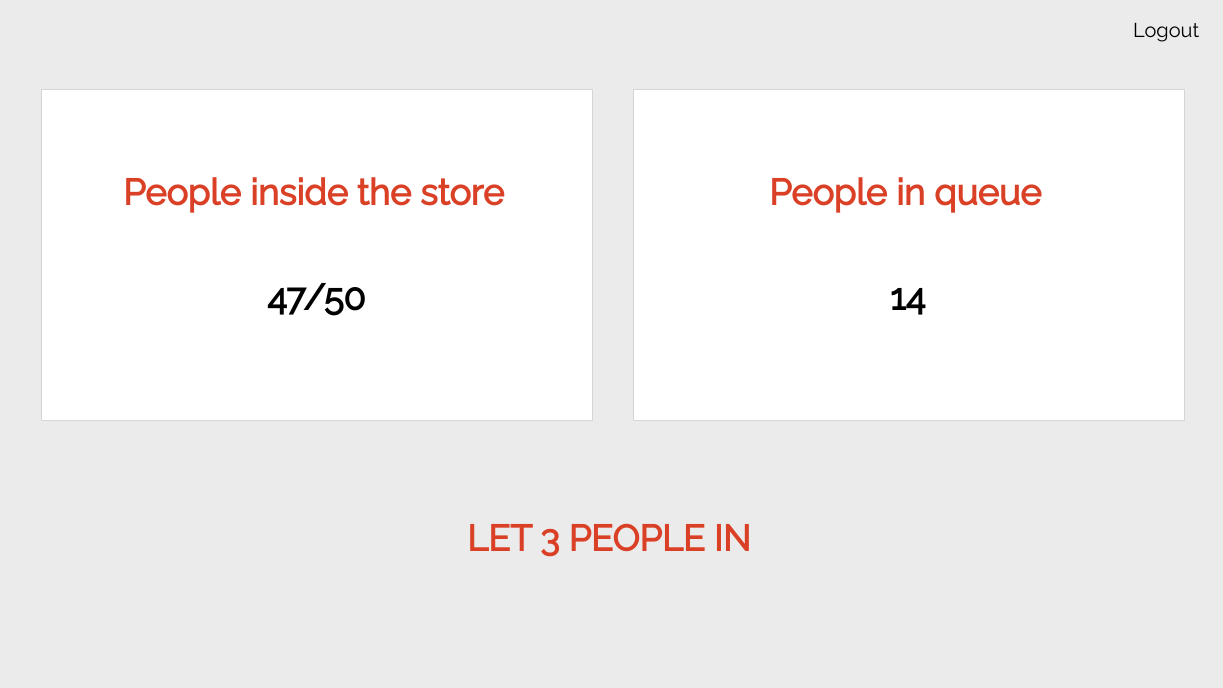
\includegraphics[width=0.64\linewidth]{employee}
	\caption{Employee homepage.}
\end{figure}
\begin{figure}[H]
	\centering
	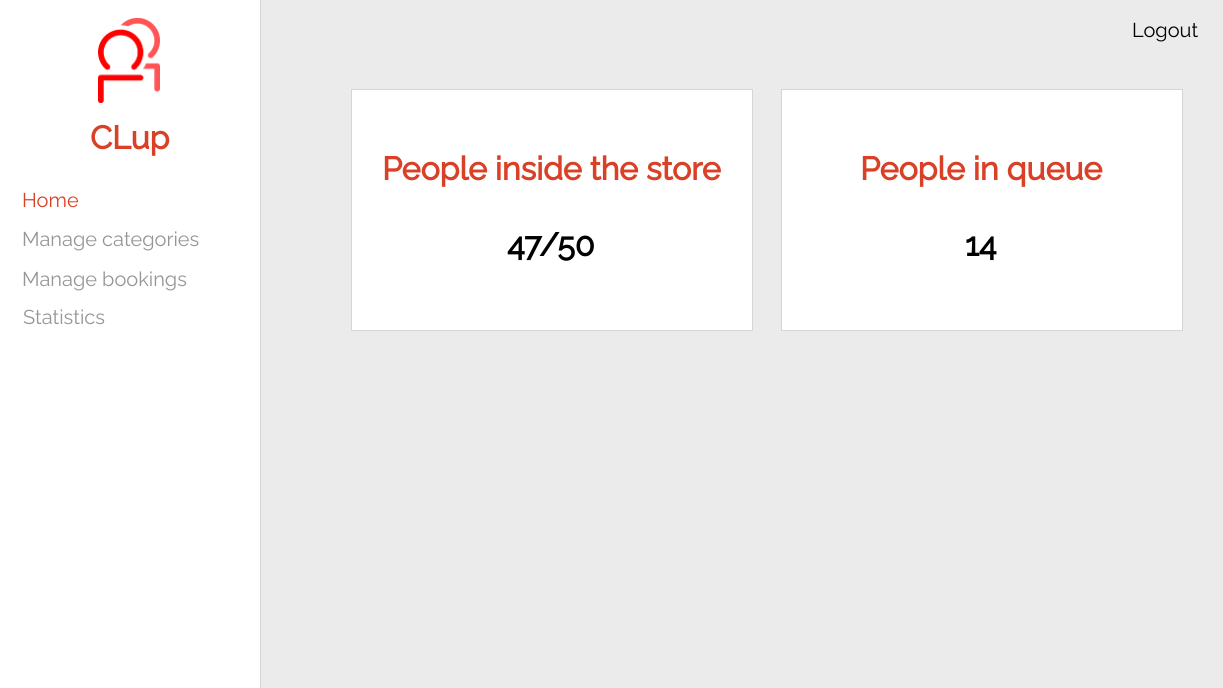
\includegraphics[width=0.64\linewidth]{dashboard1}
	\caption{Manager homepage.}
\end{figure}
\begin{figure}[H]
	\centering
	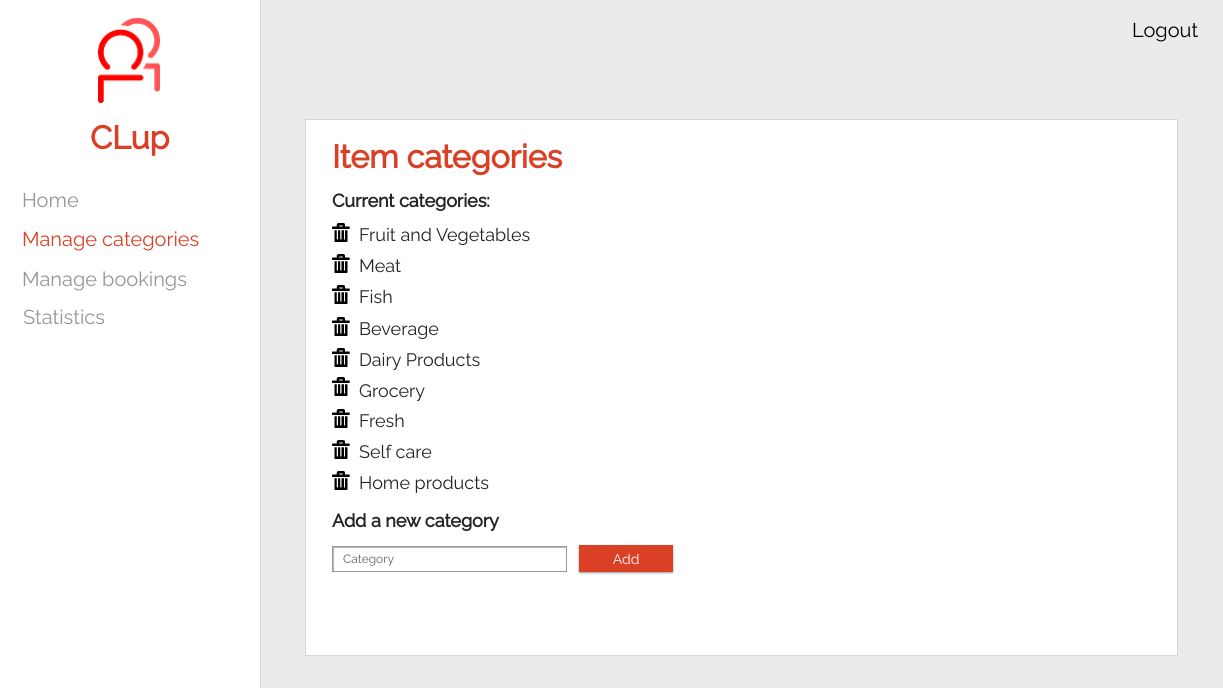
\includegraphics[width=0.64\linewidth]{dashboard2}
	\caption{Item categories page.}
\end{figure}
\begin{figure}[H]
	\centering
	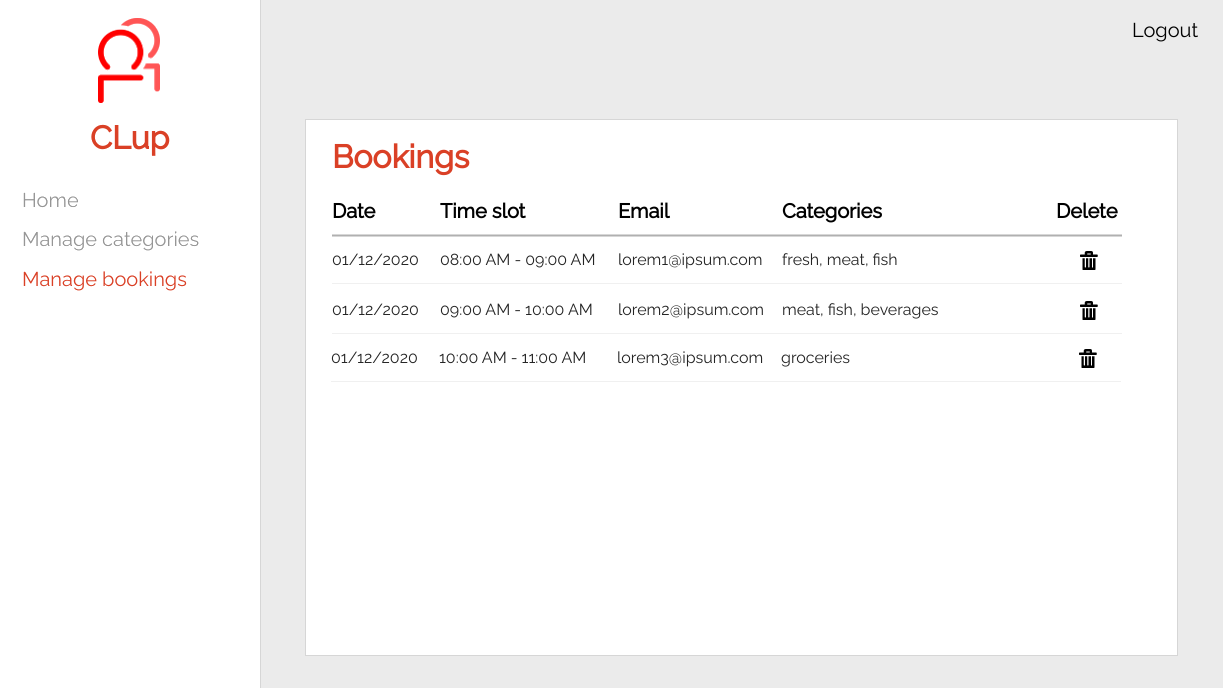
\includegraphics[width=0.64\linewidth]{dashboard3}
	\caption{Bookings list page.}
\end{figure}
\begin{figure}[H]
	\centering
	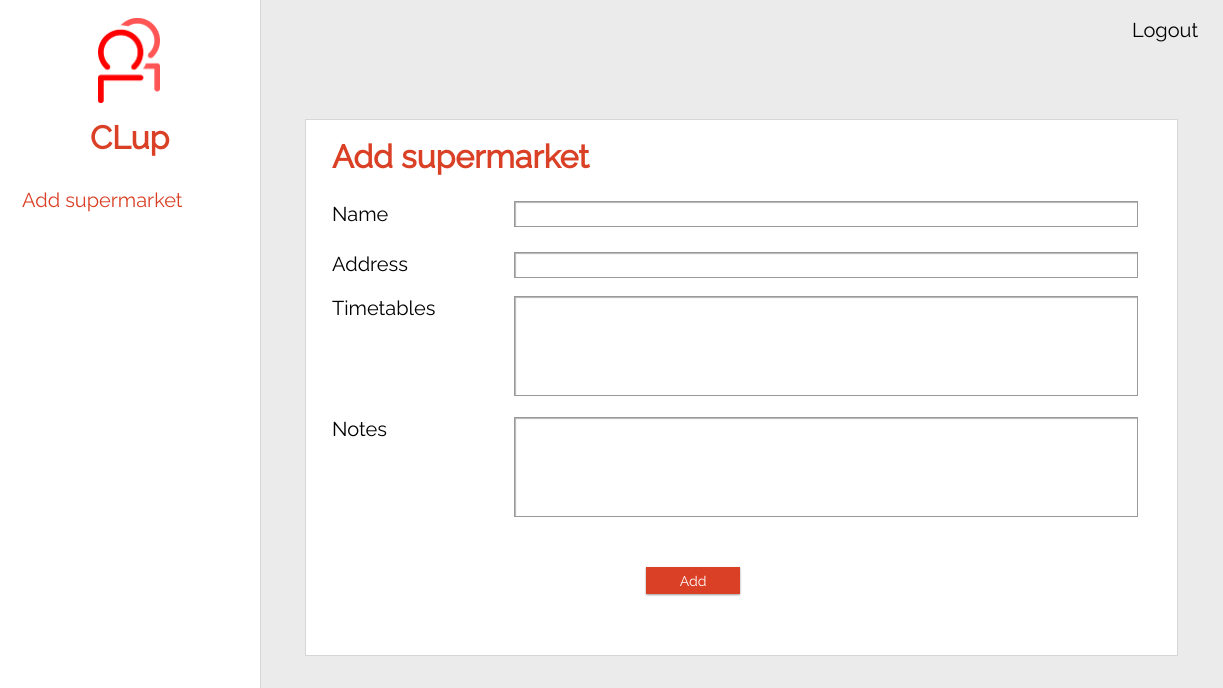
\includegraphics[width=0.64\linewidth]{new_store}
	\caption{Admin new supermarket page.}
\end{figure}

\clearpage

\subsection{User Interface Flow Diagram}
The following user interface flow diagram represent the user flow through the customer app.
\begin{figure}[H]
	\centering
	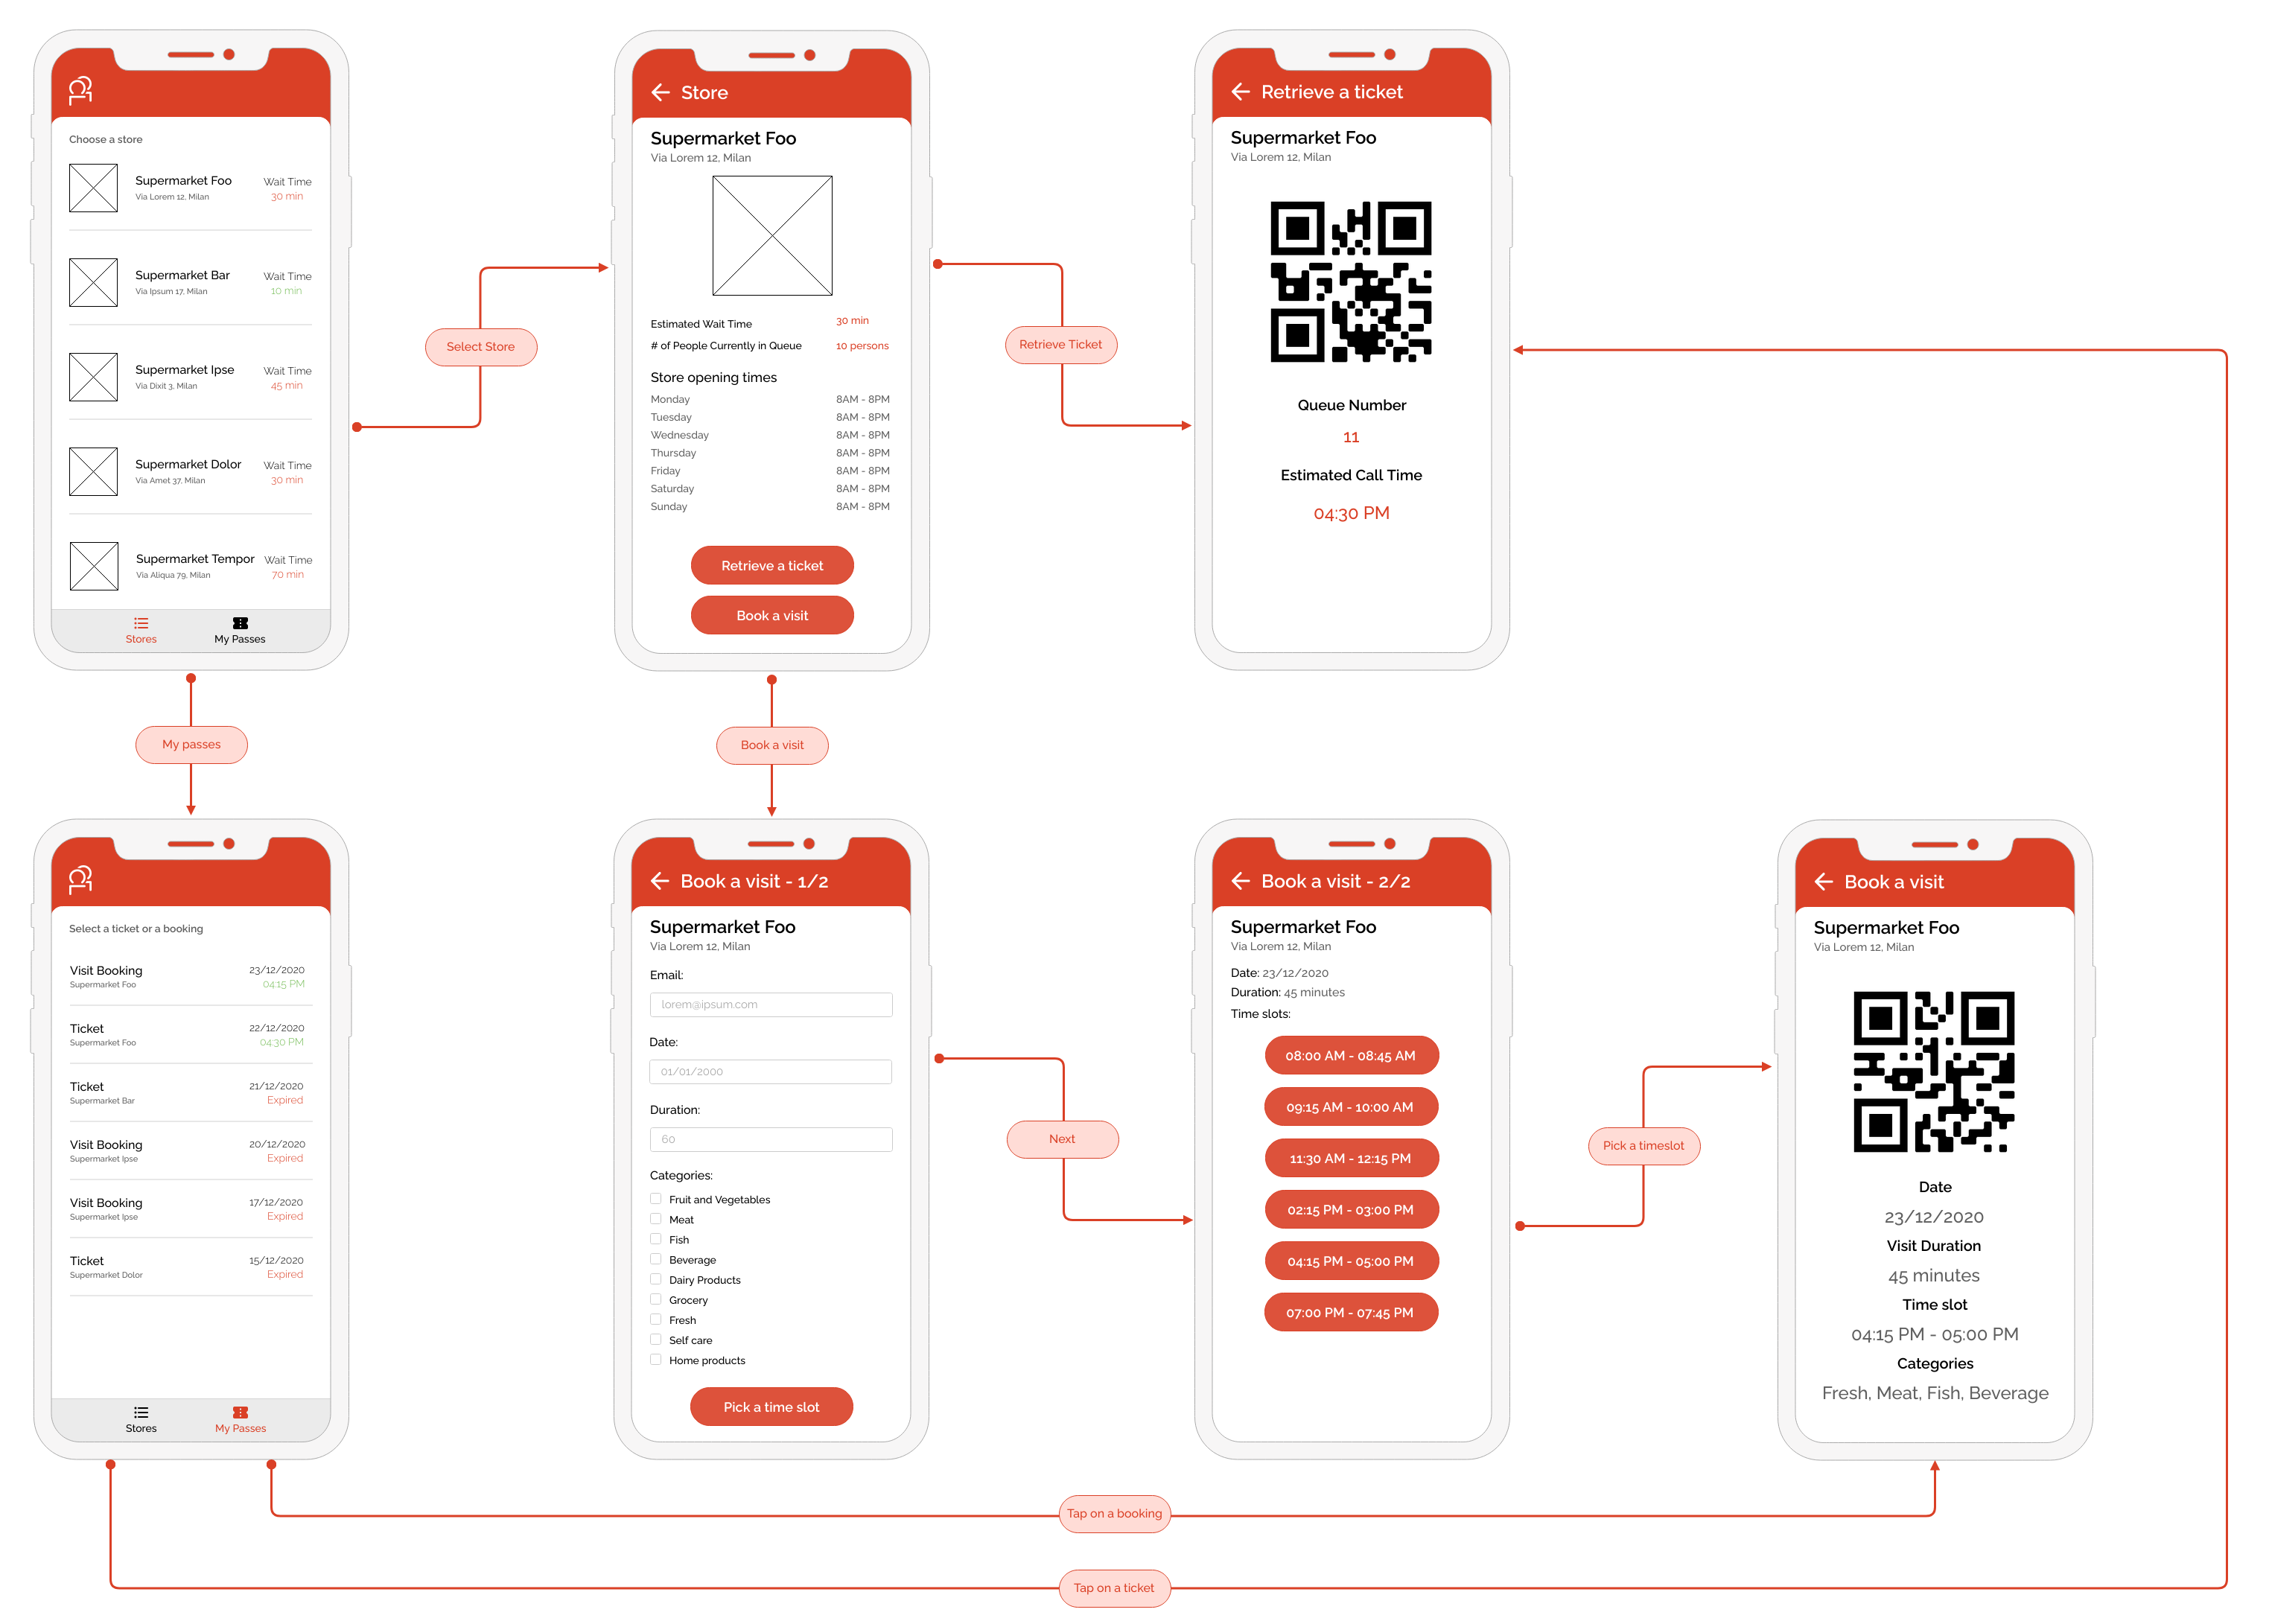
\includegraphics[width=\linewidth]{ux_flow}
	\caption{Admin new supermarket page.}
\end{figure}